\chapter{Image Acquisition and Calibration}

Since cross-talk between channels cannot be eliminated completely, there needs to be two cameras due to the way the cameras are constructed with a Bayer matrix for each pixel (see section \ref{sec:intrinsic}). Attempts to have both on a single camera are ineffective (explain why).\\

The following concepts are crucial to understand the reasoning behind certain decisions.\\

In consumer cameras, the filter pattern is arranged in an RGGB format as in Figure \ref{fig:bayer}, to mimic the physiology of the eye. Demosiacing is performed to interpolate the neighbouring pixel colours for every pixel.

\begin{figure}[H]
\centering
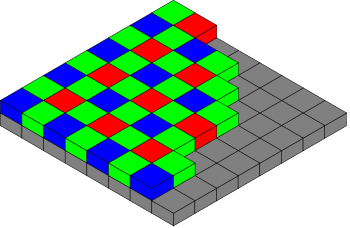
\includegraphics[scale=0.35]{images/bayer.png}
\caption{Bayer arrangement of colour filters on an image sensor's pixel array \cite{bayer}}
\label{fig:bayer}
\end{figure}

The colour filters do allow infra-red light in as well, which is why consumer cameras generally have a NIR longpass filter in place to isolate RGB colours.\\

Due to variances in focal length, and slight manufacturing disparities, there is some rotation and translation in real lenses.\\

There is also distortion, as in Figure \ref{fig:distortion_examples}.

\begin{figure}[H]
\centering
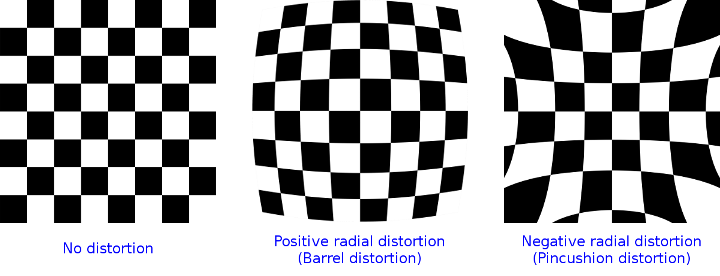
\includegraphics[scale=0.5]{images/distortion_examples.png}
\caption{Distortion examples. OpenCV \cite{calib3d}}
\label{fig:distortion_examples}
\end{figure}

This can be modelled by the pinhole camera model as in section \ref{sec:pinhole}.

%\subsection{Camera Calibration}
%
%(picture of undistortion).
%
%\subsubsection{Jello effect}
%
%ripple

\section{Pinhole Camera Model}
\label{sec:pinhole}

The cameras can be approximated as pin-hole camera models with parameters. Estimating the parameters is known as 'camera resectioning'. Light enters camera through focal point $Fc$, and falls onto the sensor, as depicted in Figure \ref{fig:camera_geometry}. $f$ is the focal length, which is the distance between the image sensor and lens. The symmetry of the model means that the correct orientation is shown at the image plane.

\begin{figure}[H]
\centering
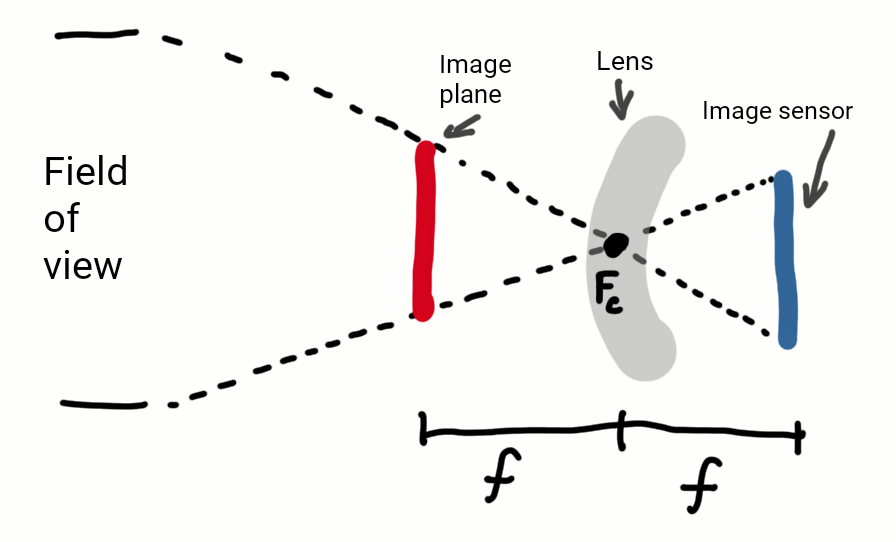
\includegraphics[scale=0.35]{images/camera_geometry.png}
\caption{Geometry of a single camera}
\label{fig:camera_geometry}
\end{figure}



\subsection{Intrinsic Parameters}
\label{sec:intrinsic}

\subsection{Extrinsic Parameters}

translation, rotation, sun, glare

\section{Filters}

A filter is needed to isolate the NIR channel. If a custom filter is used on a camera with the NIR filter removed, it is possible to isolate a NIR channel without visible light leakage on one or more colour channels. Variants include the Wratten 25A Red Long Pass filter, the Wratten 87 NIR All Pass filter and the Rosco 2008 Blue filter, which allow red and NIR light, only NIR light, and blue and NIR light respectively.\\

The Rosco 2008 Blue filter will be used, for most of the project, as well as the 600nm Dichroic Glass Longpass filter and 500nm Dichroic Glass Bandpass filter from Edmund Scientific, with limited access.

The blue Rosco 2008 filter is used as in Figure \ref{fig:blue_filter}, and passes only NIR within the green and red channels, as shown in Figure \ref{fig:blue_curve}.

\begin{figure}[H]
\begin{subfigure}{0.5\textwidth}
\centering
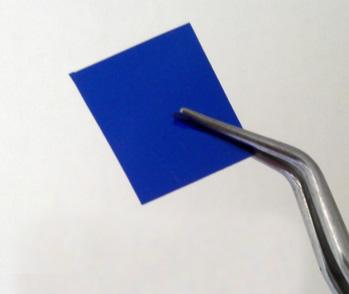
\includegraphics[scale=0.45]{images/blue_filter.jpg}
\caption{Blue Rosco 2008 filter \cite{blue_filter}}
\label{fig:blue_filter}
\end{subfigure}
\begin{subfigure}{0.5\textwidth}
\centering
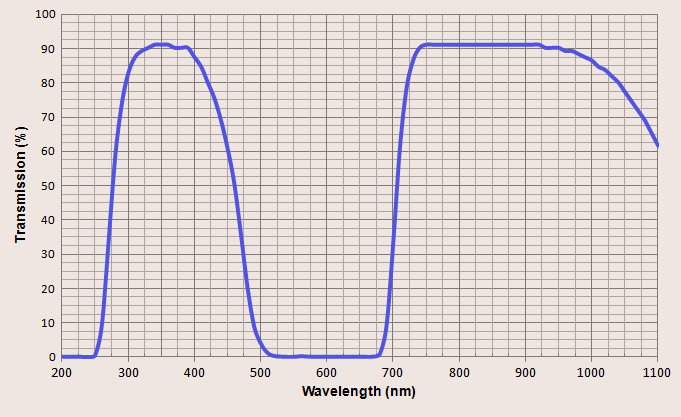
\includegraphics[scale=0.42]{images/superblueinfraredfiltercurve.png}
\caption{Blue filter transmission curve.}
\label{fig:blue_curve}
\end{subfigure}
\caption{Blue filter characteristics \cite{blue_curve}}
\label{fig:blue_character}
\end{figure}

\section{Cameras}

Two cameras are required. It is seemingly impossible to capture pure NIR and pure red on separate channels unless the intrinsic bayer matrix (see chapter 4 on intrinsic parameters) is manufactured to allow for it, however, then it would not be cost effective (citation needed).\\

The Sony IMX219 series cameras will be used. They integrate with the Raspberry Pi using a single 15-pin CSI connection.

\section{Camera mount}

The cameras will be fixed relative to each other using a PCB substrate so that no rotational or translational drift can occur.

Also, the cameras are to be dampened to prevent a jello-effect due to the rolling shutter cameras. Global shutter cameras are more expensive.

Ripple / jello

Thus, a DC brushless motorised gimbal will not be necessary.

\section{Simultaneous triggering}

A few solutions will be investigated, including the use of TCP/UDP packets and 'on the second' triggering.

Initially TCP triggering was used, but the overhead and asynchronous nature meant that it was never consistently triggered at the same time. Instead, the clocks are sychronised using NTP, and attempt to trigger every second, on the second. The latter solution works quite well, with an occassional few milliseconds difference in stereo captures.

\section{Calibration}

Stereo-calibration using 16x16 square chess board images were used.\\

Equations\\

\begin{equation}\label{eq:cm}
M_c^{(j)}\,=\,\begin{bmatrix}
{f_x^{(j)}} & {0} & {c_x^{(j)}}\\
{0} & {f_y^{(j)}} & {c_y^{(j)}}\\
{0} & {0} & {1}
\end{bmatrix},\quad j = 1,\, 2
\end{equation}

\begin{equation}\label{eq:dist}
dist\,=\,\begin{bmatrix}
k_1 & k_2 & p_1 & p_2 & k_3
\end{bmatrix}
\end{equation}

\begin{equation}\label{eq:1} R_2=R*R_1T_2=R*T_1 + T \end{equation}

\begin{equation}\label{eq:2}
E\,=\,\begin{bmatrix}
{0} & {-T_2} & {T_1}\\
{T_2} & {0} & {-T_0}\\
{-T_1} & {T_0} & {0} 
\end{bmatrix}\,*\,R
\end{equation}

\begin{align*}
F = cameraMatrix_2^{-T}\cdot E\cdot cameraMatrix_1^{-1} 
\end{align*}

\begin{align*}
T : T=[T_0, T_1, T_2]^T  
\end{align*}

\begin{equation}\label{eq:P1}
P1 = \begin{bmatrix} f & 0 & cx_1 & 0 \\ 0 & f & cy & 0 \\ 0 & 0 & 1 & 0 \end{bmatrix}
\end{equation}

\begin{equation}\label{eq:P2}
P2 = \begin{bmatrix} f & 0 & cx_2 & T_x*f \\ 0 & f & cy & 0 \\ 0 & 0 & 1 & 0 \end{bmatrix}
\end{equation}

\begin{equation}\label{eq:3}
\begin{bmatrix}{x}\\{y}\\{z}\end{bmatrix} = R  \begin{bmatrix}{X}\\{Y}\\{Z}\end{bmatrix}\,+\,t\\ \end{equation}
\begin{equation}x' = x/z \\ \end{equation}
\begin{equation}y' = y/z \\ \end{equation}
\begin{equation}x'' = x'  \frac{1 + k_1 r^2 + k_2 r^4 + k_3 r^6}{1 + k_4 r^2 + k_5 r^4 + k_6 r^6} + 2 p_1 x' y' + p_2(r^2 + 2 x'^2)  \\ \end{equation}
\begin{equation}y'' = y'  \frac{1 + k_1 r^2 + k_2 r^4 + k_3 r^6}{1 + k_4 r^2 + k_5 r^4 + k_6 r^6} + p_1 (r^2 + 2 y'^2) + 2 p_2 x' y'  \\
\quad \text{where} \quad r^2 = x'^2 + y'^2  \\ \end{equation}
\begin{equation}u = f_x*x'' + c_x \\ \end{equation}
\begin{equation}v = f_y*y'' + c_y \end{equation}

Results\\

\begin{equation}\label{eq::cm1}
M_c^1 = \begin{bmatrix}
2.523278 & 0 & 1.64 \\
0 & 2.516529 & 1.232 \\
0 & 0 & 0.001
\end{bmatrix}\cdot10^3
\end{equation}

\begin{equation}\label{eq::cm2}
M_c^2 = \begin{bmatrix}
2.505381 & 0 & 1.64 \\
0 & 2.505083 & 1.232 \\
0 & 0 & 0.001
\end{bmatrix}\cdot10^3
\end{equation}

\begin{equation}\label{eq::R}
R = \begin{bmatrix}
999.281 & -6.4992 & 37.35413 \\
6.59547 & 999.97524 & -2.45456 \\
-37.33725 & 2.69917 & 999.29908
\end{bmatrix}\cdot10^3
\end{equation}

\begin{equation}\label{eq::E}
E = \begin{bmatrix}
-0.3150989 & 158.311619 & 35.973848 \\
-55.293721 & -6.403995 & -2757.525727 \\
-18.200605 & 2753.713987 & -8.117986
\end{bmatrix}\cdot10^-3
\end{equation}

\begin{equation}\label{eq::F}
F = \begin{bmatrix}
-2.54558709\cdot10^-6 & 1.28238104\cdot10^-3 & -0.842399343\\
-0.446754\cdot10^-3 & -51.880818\cdot10^-6 & -55.4216639\\
0.1861918 & 53.846 & 1000
\end{bmatrix}\cdot10^-3
\end{equation}

\begin{equation}\label{eq::R1}
R_1 = \begin{bmatrix}
0.99977728 & 0.00654886 & -0.02006268\\
0.00657528 & 0.9999776 & -0.00125126\\
0.02005403 & 0.0013829 & 0.99979794
\end{bmatrix}
\end{equation}

\begin{equation}\label{eq::R2}
R_2 = \begin{bmatrix}
0.99826641 & 0.01319195 & -0.05735987\\
-0.01311635 & 0.99991254 & 0.00169423\\
0.05737721 & -0.00093894 & 0.99835213
\end{bmatrix}
\end{equation}

\begin{equation}\label{eq::P1}
P_1 = \begin{bmatrix}
2505.083324 & 0 & 1778.704819 & 0\\
0 & 2505.083324 & 1231.092529  & 0\\
0 & 0 & 1 & 0
\end{bmatrix}
\end{equation}

\begin{equation}\label{eq::P2}
P_2 = \begin{bmatrix}
2505.083324 &    0.       & 1778.704819 & 6909.840227\\
 0          & 2505.083324 & 1231.092529 &    0        \\
 0          &    0        &    1        &    0         \\
\end{bmatrix}
\end{equation}

\begin{equation}\label{eq::Q}
Q\ =\ \begin{bmatrix}
1 & 0 & 0 & -1.778705\cdot10^3\\
0 & 1 & 0 & -1.231093\cdot10^3\\
0 & 0 & 0 & 2.505083\cdot10^3\\
0 & 0 & -0.362539 & 0
\end{bmatrix}
\end{equation}

\begin{equation}\label{eq::T}
T\ =\ \begin{bmatrix}
2.75354568\\
0.03638771\\
-0.15821732
\end{bmatrix}
\end{equation}

\begin{equation}\label{eq::validpix1}
valid\ Pix\ ROI_1\ =\ 
\begin{bmatrix}
x_1 & y_1\\
x_2 & y_2
\end{bmatrix}\ =
\begin{bmatrix}
88 & 6\\
3192 & 2421
\end{bmatrix}
\end{equation}

\begin{equation}\label{eq::validpix2}
valid\ Pix\ ROI_2\ =\ 
\begin{bmatrix}
x_1 & y_1\\
x_2 & y_2
\end{bmatrix}\ =
\begin{bmatrix}
0 & 26\\
3204 & 2378
\end{bmatrix}
\end{equation}

\begin{equation}\label{eq::error1}
error_1 = 17.255\%
\end{equation}
\begin{equation}\label{eq::error2}
error_2 = 14.647\%
\end{equation}


\subsection{Calibration Technique}

\subsection{Measured Results}

\section{Stereo-rectification}

The images were undistorted (see chapter 4 on intrinsic parameters) according to the simultaneous chess board images it was calibrated at.

\subsection{Measured Results}